\chapter{Objeto}
\section{Laboratório Ocean}

De forma a se aproximar de um dos principais nichos de seu interesse, a Samsung criou um programa de Relacionamento com Desenvolvedores, de forma a se aproximar de um grupo de profissionais que mais contribuem com a disseminação de novas tecnologias da Samsung. Esse programa possui diversas frentes, como o \textit{Developer Day}, que é um grande evento realizado uma vez por ano no Brasil e outros países da América Latina que visa promover as mais recentes tecnologias da marca, e o Laboratório Ocean, que visa a aproximação da comunidade estudantil e de startups em formação.

O Laboratório Ocean é uma iniciativa da Samsung que consiste em estimular desenvolvedores a criar soluções tecnológicas relacionadas aos produtos da marca coreana. A primeira sede do laboratório foi inaugurada em 2010 na Coréia do Sul, e a iniciativa foi replicada no Brasil há cerca de dois anos, com uma unidade em Manaus e outra em São Paulo. Ao passo que a unidade de Manaus foi estabelecida dentro da Universidade Estadual do Amazonas (UEA), a unidade de São Paulo encontrava-se até o fim de 2015 na Avenida Brigadeiro Faria Lima, uma das principais avenidas comerciais da cidade. Uma iniciativa recente movida por um ex-aluno, professores do departamento e o programa 'Parceiros da Poli' trouxe através de conversas informais a ideia de trazer o laboratório para dentro da USP. Como o modelo intra universitário funcionou bem em Manaus, foi decidido replicar o modelo e sediar o laboratório dentro da Universidade, hospedado dentro do Departamento de Engenharia de Produção (PRO).

A infraestrutura do laboratório consiste em uma grande sala para até 80 pessoas, porém caso necessário portas retráteis permitem a sua divisão em duas salas separadas. Essa estrutura fica aberta das 08 às 22 horas de segunda a sexta feira, podendo ser utilizada livremente pela comunidade estudantil da universidade, cedendo computadores e acesso a Wi-Fi de alta velocidade. As mesmas salas também são utilizadas para a realização de cursos ministrados gratuitamente pela Samsung e abertos à comunidade.

Basicamente são fornecidos dois tipos de cursos, básicos e intensivos. Os cursos básicos são de curta duração (aproximadamente 3 horas), e os cursos intensivos em seu módulo atual duram 4 meses, utilizando o espaço toda noite de segunda à quinta-feira. O foco inicial dos cursos foi o desenvolvimento em dispositivos móveis, em especial apoiados no sistema operacional Android, pois é o que roda nos aparelhos da Samsung, como o Galaxy S7. Com o passar do tempo, os cursos começaram a seguir as tendências de hardware de interesse do mercado e da própria Samsung, como \textit{wearables}, \textit{smart} TVs, Internet das Coisas e Realidade Virtual. Mesmo assim, a área de dispositivos móveis ainda representa 80\% dos cursos oferecidos por eles.

Os cursos curtos possuem como principal objetivos despertar o interesse de desenvolvedores em relação aos produtos da Samsung. Para tal, os cursos trabalham de forma a mostrar todos os produtos de alta tecnologia da samsung e capacitar desenvolvedores para que utilizem os seus dispositivos através de software. Para tal, é disseminado tanto o funcionamento dos \textit{Software Development Kits} (SDKs) da Samsung e suas APIs para permitir o acesso ao \textit{hardware} dos seus dispositivos quanto o uso do Android para manipulação do software na linguagem nativa atual do sistema operacional utilizado por eles. Para a execução desses cursos, a Samsung trabalha juntamente com empresas terceiras especialistas no assunto para preparar o material a ser passado. Algumas vezes funcionários da própria Samsung dão o treinamento, e em alguns momentos houve até participação do corpo docente da Poli.

Os cursos intensivos são cursos de pré-aceleração de empresas, e têm o intuito de fomentar o empreendedorismo, apesar de manter a base de disseminar o conhecimento em cima de produtos da Samsung. A empresa acredita que no atual mercado, a diferenciação sobre o \textit{hardware} está ficando cada vez mais difícil, por isso as empresas estão buscando se diferenciar frente às outras em conteúdo. Dentro desse contexto, a Samsung visa auxiliar empresas a se desenvolverem e elas - em contrapartida - auxiliam a enriquecer dos produtos da Samsung, seja através de novos produtos ou através de serviços.

Dessa forma, os cursos de pré-aceleração procuram fornecer conhecimento e experiência ao desenvolvimento de suas empresas, através de mentorias, bate-papo, palestras e avaliações. Como são cursos gratuitos, um dos principais desafios é manter o próprio engajamento das empresas, por isso o motivo de haver encontros 4 vezes por semana, com mentoria, criação e gestão do projeto proposto pelo programa, com checkpoints de avaliação das empresas ao longo do projeto. Tudo isso feito de forma \textit{gamificada} dentro do próprio modelo. A prrimeira parte do programa consiste da validação do modelo de negócio proposto pela empresa, e a segunda parte corresponde a prototipação e desenvolvimento de produto de fato. Participam desse programa profissionais da Samsung, funcionários terceiros, professores da USP, membros do NEU e empresas parceiras (Sebrae, FIESP, IBM, Amazon).

Por se tratar de um acordo entre a Samsung e o PRO, é necessário que sejam feitas reuniões de alinhamento das necessidades e expectativas entre partes, que não estão sendo realizadas nesse primeiro momento pois o projeto ainda está no início e não há conflitos aparentes. Entretanto a universidade também tem planos para o laboratório e acredita que o mesmo terá um grande impacto dentro e fora da universidade. Segundo as palavras do professor Eduardo Zancul na inauguração do Ocean: “É uma frente de ensino, pesquisa e extensão. Ensino pois será um espaço para disciplinas do curso de engenharia de produção; Pesquisa porque materiais e a estrutura do laboratório serão utilizados pela comunidade acadêmica; Extensão pois muitos cursos serão abertos para a comunidade”. O laboratório se tornou uma parceria de cogestão entre universidade e empresa que tem como principal mérito a geração de valor derivada da sinergia entre academia e indústria. 

\section{Identificação de Stakeholders do Laboratório}
\label{sec:identificacao_stakeholders}

De forma a ilustrar os principais stakeholders do laboratório representados nesse trabalho, foi criado um mapa representativos dos mesmos. 

\begin{figure}[h]
\caption{Mapa de stakeholders do projeto Ocean}
\centerline{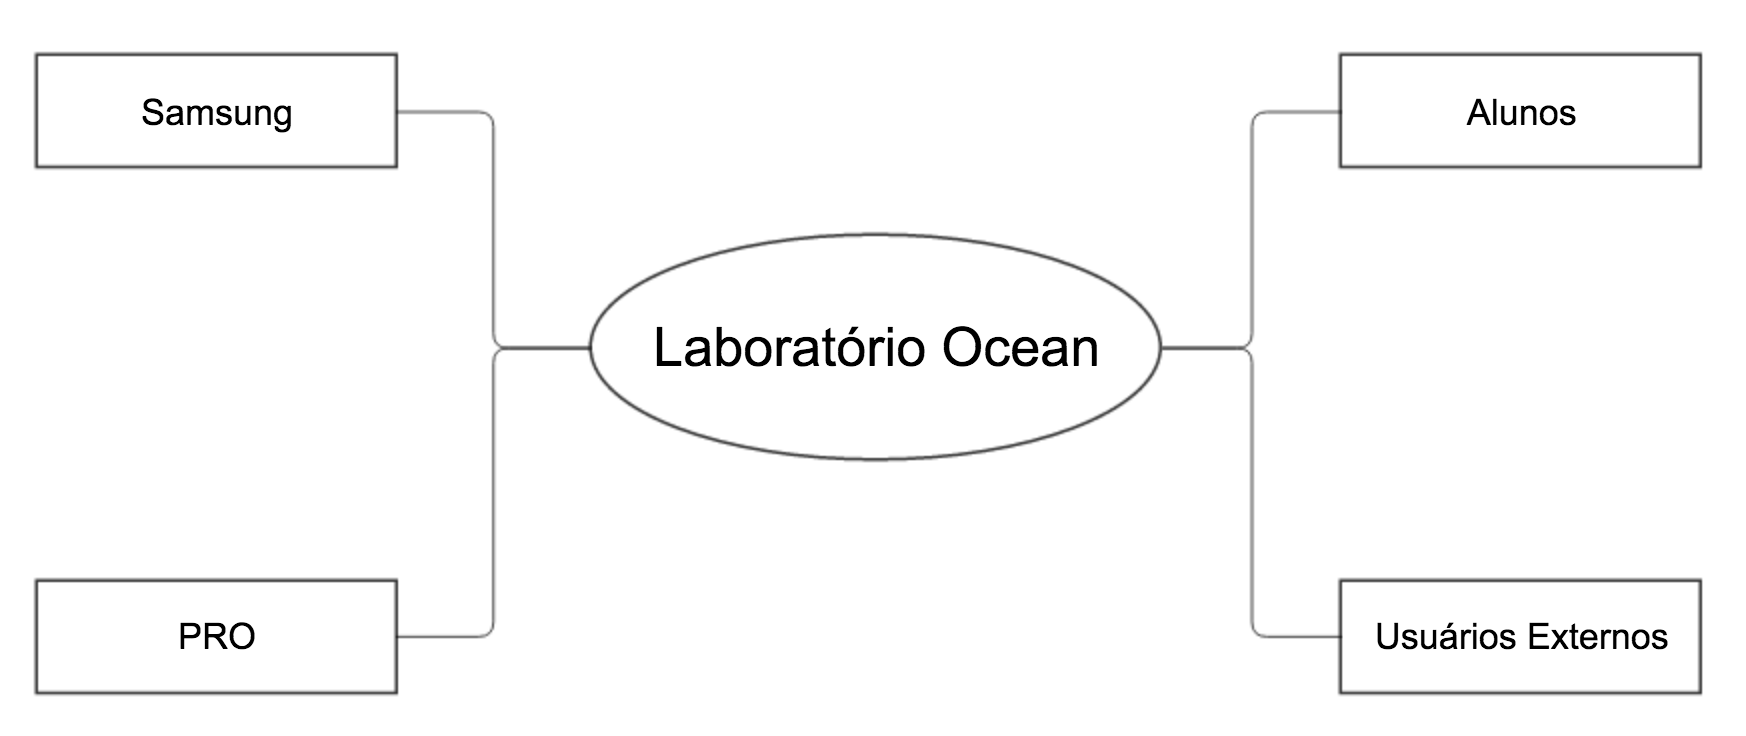
\includegraphics[scale=0.5]{img/stakeholders}}
\label{fig:stakeholders}
\caption* {Fonte: Elaborado pelo próprio autor}
\end{figure}

\subsection{PRO}
\label{sec:con_pro}

O Ocean é um dos quatro grandes projetos que o PRO acompanha atualmente, esquematizado pela Tabela \ref{tab:pilares_pro}, juntamente com Inovalab, a Fábrica Didática e o Núcleo de Empreendedorismo da USP.

\begin{table}[H]
\begin{center}
\caption{Pilares do PRO}
\label{tab:pilares_pro}
{\def\arraystretch{2}\tabcolsep=10pt
\begin{tabular}{>{\raggedright}p{0.2\linewidth}>{\raggedright\arraybackslash}p{0.2\linewidth}>{\raggedright\arraybackslash}p{0.2\linewidth}>{\raggedright\arraybackslash}p{0.2\linewidth}}
\hline
     & Objetivo Institucional & Participação do PRO & Em Atividade  \\ \hline
     Inovalab & Laboratório de Inovação & Gestão Ativa & Sim  \\
     Fábrica Didática & Apropriação de conceitos de fábricas para aplicação no ensino & Em Desenvolvimento & Não \\
     Ocean & Laboratório de Desenvolvimento de Software & Cogestão com a Samsung & Sim \\
	 Núcleo de Empreendedorismo da USP & Disseminação da cultura empreendedora & Cede espaço físico & Sim \\ \hline
\end{tabular}%
}
\caption* {Fonte: Elaborado pelo autor em conversa com professores do departamento}
\end{center}
\end{table}

//Falar um pouco sobre cada um desses projetos, dar mais volume e explicar a importância do Ocean dentro desse contexto. 


Segundo \citeonline{jeeModels}, o ensino de engenharia pode ser dividido em 3 principais modelos: Acadêmico, Market-Driven e Integrativo.

\begin{table}[H]
\begin{center}
\caption{Modelos de ensino de engenharia}
\label{tab:modelos_ensino_tab}
{\def\arraystretch{2}\tabcolsep=10pt
\begin{tabular}{>{\raggedright}p{0.2\linewidth}>{\raggedright\arraybackslash}p{0.2\linewidth}>{\raggedright\arraybackslash}p{0.2\linewidth}>{\raggedright\arraybackslash}p{0.2\linewidth}}
\hline
     & Modelo Acadêmico & Modelo \textit{Market-Driven} & Modelo Integrativo \\ \hline
     Percepção de Engenharia & Ciência Aplicada & Inovação Tecnológica & Serviço Público \\
     Papel Social & Consultor, Especialista & Empreendedor, Gestor & Cidadão, Agente de Mudanças \\
     Perspectiva Institucional & Universidade Científica & Universidade Empreendedora & Universidade Ecológica  \\
	 Exemplos de Disciplinas & Cálculo, Estatística & Empreendedorismo, Desenvolvimento de Produto & Sustentabilidade, Problemas da Sociedade \\ \hline
\end{tabular}%
}
\caption* {Fonte: Adaptado de \citeonline{jeeModels}}
\end{center}
\end{table}

Dentro desse contexto, é possível observar uma grande sinergia entre o laboratório e o modelo \textit{Market-Driven}, pois o departamento pode o utilizar para auxiliar no desenvolvimento de engenheiros para estarem alinhados com as necessidades do mercado, sendo este representado por uma das empresas com maior tecnologia de ponto a nivel global.

\subsection{Alunos}
\label{sec:con_alunos}

A presença de um laboratório como este também ajuda a fomentar a cultura de empreendedorismo dentro da universidade, pois deixa os alunos próximos ao desenvolvimento de software, uma das principais bases de criação de novas \textit{startups}, devido ao baixo custo de aprendizado e investimento e alto valor gerado no curto e médio prazo. Ainda, segundo \citeonline{entrepreneurship}, os estudantes de engenharia experienciam o empreendedorismo de 4 maneiras: 

\begin{enumerate}
\item Primeiro passo para o auto-aprendizado
\item Preparação para a vida no trabalho
\item Caminho para ser autônomo
\item Desenvolvimento de liderança e responsabilidade de um time
\end{enumerate}

\subsection{Usuários Externos}
\label{sec:con_usuarios}

Segundo a 27\textsuperscript{a} Pesquisa de Anual do uso de TI, realizada pela Fundação Getúlio Vargas (FGV), o número de smartphones em uso no Brasil gira atualmente em torno de 168 milhões de dispositivos. \cite{tifgv} Não obstante, além do alto número de smartphones, o Brasil também se mostra presente no mercado de outros dispositivos inteligentes, com previsão de movimentação de US\$4,1 bilhões no Brasil com IOT, segundo a assessoria de imprensa da IDC Brasil. \cite{idc}

É nesse cenário de alto crescimento do uso de novas tecnologias no Brasil que o mesmo se mostra como um grande mercado para produtos inerentes ao uso de dispositivos inteligentes, como aplicativos e games. Dentro desse contexto, jovens interessados pelo desenvolvimento desse mercado no país podem utilizar o Ocean para realizar diferentes cursos nessas áreas, desde aulas para iniciantes até cursos mais avançados.

Além do uso aplicado diretamente nessa área de dispositivos portáteis, a programação desenvolvida nessas atividades pode ser extendida para outras áreas de desenvolvimento, tornando os jovens mais capacitados para qualquer área tecnológica. Segundo a ONG Code.org, financiada por fundadores das maiores empresas de tecnologia do mundo como Mark Zuckerberg e Bill Gates, o número de empregos para programadores cresce exponencialmente, ao passo que o ensino de programação nas escolas não acompanha o mesmo ritmo, o que gerará uma falta de profissionais de TI em um futuro próximo. Juntamente a essa informação, o departamento de estatísticas de trabalho dos Estados Unidos (\textit{Bureau of Labor Statistics}) estima que o número de empregos para programadores dentro dos EUA diminuirá em até 8\%, pois mais profissionais deverão ser recrutados fora do país, devido ao baixo custo e a flexibilidade de trabalho remoto permitida pela programação. \cite{bls}